\documentclass[12pt,a4paper]{article}
\usepackage[utf8]{inputenc}
\usepackage[german]{babel}
\usepackage[T1]{fontenc}
\usepackage{amsmath}
\usepackage{amsfonts}
\usepackage{amssymb}
\usepackage{graphicx}
\usepackage{siunitx}
\usepackage{float}
\usepackage[left=2cm,right=2cm,top=2cm,bottom=2cm]{geometry}
\author{Gerald}

\begin{document}
\sisetup{separate-uncertainty = true}
	\setlength{\parindent}{0pt} 
	\begin{center}
		{\LARGE Versuchsprotokoll}\\
		\begin{large}
			zum Fortgeschrittenenpraktikum im Bachelorstudiengang Physik\\[0.4cm]
			an der RWTH Aachen\\
			II. Physikalisches Institut A\\[5.5cm]
			\Large\textbf{\textsl{Rastertunnelmikroskopie (STM)}}\\[5.5cm]
			\normalsize\textit{vorgelegt\\von}\\[0.4cm]
			\large{Moritz Berger (355244)\\Gerald Kolter (355005)}\\Gruppe 30\\[2cm]
			\large \textbf{Wintersemester 2017/18}
		\end{large}
	\end{center}
	\newpage
	
	\tableofcontents
	\newpage

\section{Versuchsziel}
Das Ziel des Versuchs besteht darin, mit einem Rastertunnelmikroskop bei der Vermessung einer Goldprobe die Auswirkung der Einstellungen auf das Messergebnis zu untersuchen. Mit einer Probe eines hochorientierten pyrolytischen Graphit (HOPG) wird der Abstand der Gitterebenen bestimmt und eine Kalibration in x- und y-Richtung durchgeführt.

\section{Aufbau}
Das verwendete Rastertunnelmikroskop besteht aus einem Halter für die Platin-Iridium-Spitze, der mit piezoelektrischen Kristallen in allen drei Raumrichtungen bewegt werden kann, und einem Probenhalter, der auf einem sogenannten Schrittmotorantrieb liegt. Dieser funktioniert ebenfalls mit einem piezoelektrischen Kristall und dient lediglich der Grobannäherung. Spitze und Probe sind über eine Spannungsquelle verbunden, wobei gleichzeitig der in diesem Kreis fließende Strom gemessen wird. Dieser Strom kommt bei kleinen Abständen zwischen Spitze und Probe durch den Tunneleffekt zustande. Die Abhängigkeit zwischen Strom und Abstand ist exponentiell und damit sehr stark.\\
Die Spitze wird mit den piezoelektrischen Kristallen über die Probe gerastert, wobei jede Linie in x-Richtung vorwärts und rückwärts abgefahren wird.\\
Eine Regelungselektronik steuert die z-Richtung der Spitze in Abhängigkeit des Tunnelstroms. Dabei gibt der sogenannte I-Gain an, wie schnell die Regelung auf kurze Pulse reagiert.

\section{Durchführung}
\subsection{Untersuchung der Mikroskopeigenschaften mit einer Goldprobe}
\subsection{Untersuchung von HOPG}

\subsubsection{Korrektur der Achsen über Atomabstände}
Die Achsenkalibration findet anhand der atomaren Abstände des Graphit-Gitters statt.\\

\begin{table}
\centering
\begin{tabular}{|c|c|c|c|c|}
\hline 
Modus & Bereichsgröße[nm] & Zeilenzeit[s] & IGain & Spannung[mV]\\ 
\hline 
Höhen & 1 & 0.3 & 100 & 50.4\\ 
\hline 
Höhen & 2.325 & 0.3 & 100 & 50.4\\ 
\hline 
Höhen & 5 & 0.3 & 100 & 50.4\\ 
\hline 
Strom & 0.872 & 0.2 & 8000 & 50.4\\ 
\hline 
Strom & 2.325 & 0.2 & 8000 & 50.4\\ 
\hline 
Strom & 5 & 0.2 & 8000 & 50.4\\ 
\hline 
\end{tabular} 
\caption{Messeinstellungen aller Aufnahmen zu den Atomabständen.}
\label{tab:Atome_Einstellungen}
\end{table}

\section{Ergebnisse}
\subsection{Untersuchung der Mikroskopeigenschaften mit einer Goldprobe}

\subsection{Untersuchung von HOPG}
\subsubsection{Kalibration der Achsen}

\begin{figure}
\centering
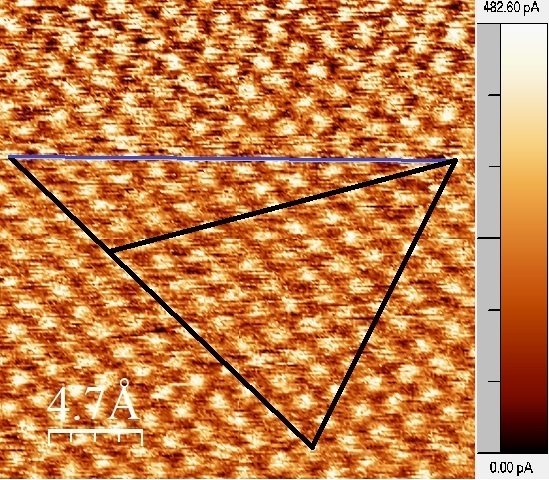
\includegraphics[scale=0.9]{Bilder/Atome/hoch2_h_scale.jpg}
\caption{Methode zur Bestimmung der x-Korrektur}
\label{fig:hoch2_h}
\end{figure}

\begin{figure}
\centering
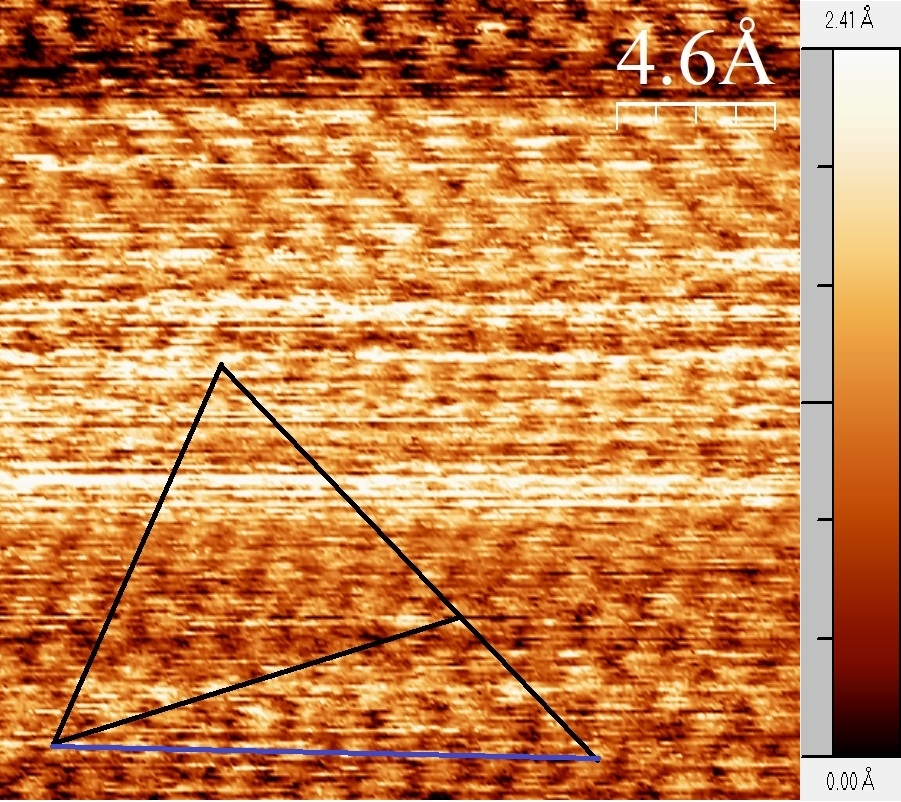
\includegraphics[scale=0.54]{Bilder/Atome/strom2_h_scale.jpg}
\caption{Methode zur Bestimmung der x-Korrektur}
\label{fig:strom2_h}
\end{figure}

Um die Längenskalen in x- und y-Richtung möglichst unkorreliert kalibrieren zu können, kann nicht direkt der Atomabstand benutzt werden. Stattdessen wird der Abstand zwischen 2 Atomen bestimmt, die möglichst auf einer der beiden Achsen liegen. Dann wird über ein Dreieck entlang der Symmetrieachsen des Atomgitters die echte Länge dieses Abstandes bestimmt.\\
Dies ist möglich, da man aus der Gitterstruktur den Winkel zwischen den Symmetrieachsen($60^{\circ}$) und die Atomabstände (\SI{2.46}{\angstrom}) und damit die Längen entlang der Achsen kennt. Man kann also die Atome entlang des Dreieckes zählen daraus über den allgemeinen Satz von Pythagoras die Länge in die Achsenrichtung bestimmen:
\begin{equation}
c = \sqrt{(a\cdot n)^{2}+(a\cdot m)^2-2 a^{2}\cdot n\cdot m\cdot cos(\alpha)}
\end{equation}
Hierbei ist c die zu bestimmende Länge, a die Atomlänge, n und m die Anzahl der Atome entlang einer Dreiecksseite und $\alpha$ der Winkel zwischen diesen Seiten.\\
In Abbildung \ref{fig:hoch2_h} und \ref{fig:strom2_h} ist diese Methode beispielhaft anhand den 2.325nm Messungen gezeigt.\\
Vor allem bei kleineren Zoomstufen konnte oft die Anzahl der Atome nicht mit 100\% Genauigkeit bestimmt werden.
Um mögliche Zählfehler erkennen zu können wurde deswegen sowohl einmal über die  $60^{\circ}$-Symmetrie, als auch einmal über $120^{\circ}$-Symmetrie die Länge bestimmt. Diese Längen sollten identisch sein. Wenn dies nicht der Fall ist, hat man sich offensichtlich verzählt.\\
Die Atome waren manchmal sehr schwer zu erkennen, weswegen stattdessen die Anzahl oft anhand der durchquerten Symmetrieachsen bestimmt wurde. Dies ist schematisch in Abbildung \ref{fig:strom5_symmetire} dargestellt.\\
\\
Es muss außerdem noch die gemessene Länge von c im Bild bestimmt werden.\\
Dazu wird an insgesamt 6 verschiedenen Stellen der Abstand zwischen zwei Atomen gemessen, die die gleiche Anzahl von Atomen zwischen sich liegen haben.
Dies ist ebenfalls schematisch in Abbildung \ref{fig:strom2_abstand} dargestellt.\\
Die so erhaltenden Längen wurden gemittelt. Daraus erhält man auch einen Fehler auf die Längen.\\
\\
Mit diesem Verfahren wurden alle 6 Messungen jeweils unabhängig für die x- und y-Richtung ausgewertet. Die Ergebnisse sind in Tabelle \ref{tab:Atome_horizontal} für die x-Richtung und in Tabelle \ref{tab:Atome_vertikal} für die y-Richtung zusammengefasst.\\
Die restlichen Bilder, die zur Auswertung benutzt wurden, befinden sich im Anhang.\\


\begin{figure}
\centering
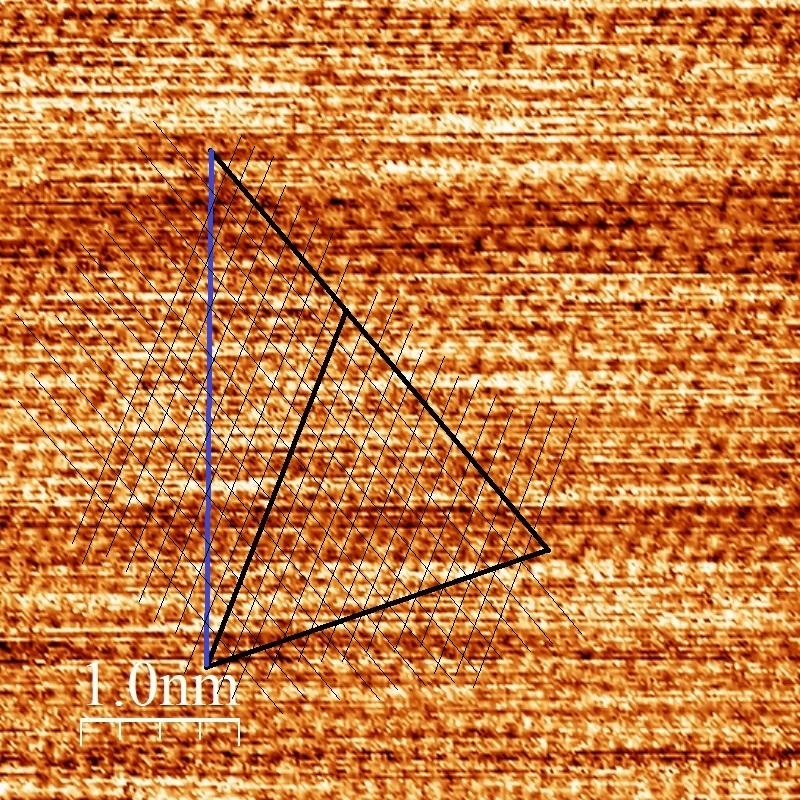
\includegraphics[scale=0.6]{Bilder/Atome/strom5_v_gitter.jpg}
\caption{Darstellung des sichtbaren Atomgitters anhand der 5nm Strommessung, um das Ablesen der Atomanzahl zu vereinfachen.}
\label{fig:strom5_symmetire}
\end{figure}

\begin{figure}
\centering
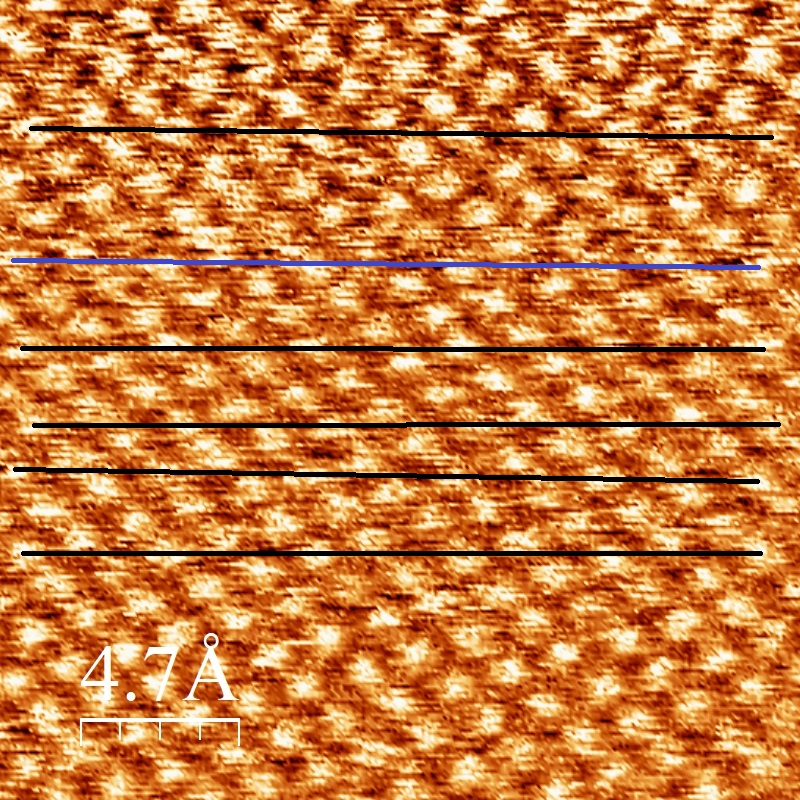
\includegraphics[scale=0.54]{Bilder/Atome/hoch2_abstand.jpg}
\caption{Beispielhafte Auswahl von 6 Abständen, die den Originalabstand(blau) repräsentieren. Die Abstände wurden gemittelt, um die gemessene Länge bestimmen zu können.}
\label{fig:strom2_abstand}
\end{figure}


\begin{table}
\begin{tabular}{|c|c|c||c|c||c|c|}
\hline 
Modus & Bildbreite [\si{\angstrom}] & Abstand [\si{\angstrom}] & Atome($60^{\circ}$) & Atome($120^{\circ}$) & berechn. Länge [\si{\angstrom}] & rel. Länge\\ 
\hline 
\hline 
Höhen & 10 & $8.81\pm 0.04$ & 6/4 & 2/4 & 13.02& 1.478/0.677\\ 
\hline 
Höhen & 23.25 & $21.50\pm 0.04$ & 10/15 & 10/5 & 32.54& 1.513/0.661\\ 
\hline 
Höhen & 50 & $18.4\pm 0.07$ & 4/6  & 4/2 & 28.38& 1.542/0.648\\ 
\hline 
\hline
Strom & 8.719 & $6.07\pm 0.03$ & 4/6 & 4/2 & 8.87& 1.461/0.684\\ 
\hline 
Strom & 23.25 & $16.74\pm 0.14$ & 7/11  & 7/4 & 23.72& 1.417/0.706\\ 
\hline 
Strom & 50 & $40.00\pm 0.09$ & 19/28  & 19/9 & 60.91& 1.523/0.657\\ 
\hline 
\end{tabular} 
\caption{Ergebnisse der \textbf{horizontalen} Längenmessung. Angegeben ist der verwendete Modus(Konstanthöhen-/Konstantstrommodus), die Bildbreite, der abgelesene Abstand, die Anzahl der Atome über einen $60^{\circ}$/$120^{\circ}$ Winkel, die daraus berechnete Länge und das Verhältnis von berechneter zur abgelesenen Länge.}
\label{tab:Atome_horizontal}
\end{table}

\begin{table}
\begin{tabular}{|c|c|c||c|c||c|c|}
\hline 
Modus & Bildbreite [\si{\angstrom}]  & Abstand [\si{\angstrom}] & Atome($60^{\circ}$) & Atome($120^{\circ}$) & berechn. Länge [\si{\angstrom}] & rel. Länge\\ 
\hline 
\hline 
Höhen & 10 & $8.55\pm 0.04$ & 5/4 & 5/9 & 19.21& 2.247/0.445\\ 
\hline 
Höhen & 23.25 & $20.81\pm 0.06$ & 10/17  & 10/7 & 36.40& 1.749/0.572\\ 
\hline 
Höhen & 50 & $22.88\pm 0.17$ & 10/17  & 10/7 & 36.40& 1.591/0.629\\ 
\hline 
\hline 
Strom & 8.719 & $6.18\pm 0.06$ & 3/2 & 3/5 & 10.72& 1.735/0.576\\ 
\hline 
Strom & 23.25 & $18.00\pm 0.07$ & 8/14  & 8/6 & 29.93& 1.663/0.601\\ 
\hline 
Strom & 50 & $32.22\pm 0.15$ & 13/22  & 13/9 & 47.13& 1.462/0.684\\ 
\hline 
\end{tabular} 
\caption{Ergebnisse der \textbf{vertikalen} Längenmessung. Angegeben ist der verwendete Modus(Konstanthöhen-/Konstantstrommodus), die Bildbreite, der abgelesene Abstand, die Anzahl der Atome über einen $60^{\circ}$/$120^{\circ}$ Winkel, die daraus berechnete Länge und das Verhältnis von berechneter zur abgelesenen Länge.}
\label{tab:Atome_vertikal}
\end{table}

Anhand dieser Daten wird nun eine lineare Regression durchgeführt, aus dessen Steigung der Korrekturfaktor bestimmt wird.\\
Daraus ergeben sich folgende Korrekturfaktoren:
\begin{equation*}
\boxed{\textrm{horizontale Korrektur}: 1.511\pm 0.015}
\end{equation*}

\begin{equation*}
\boxed{\textrm{vertikale Korrektur}: 1.599\pm 0.072}
\end{equation*}

\begin{figure}
\centering
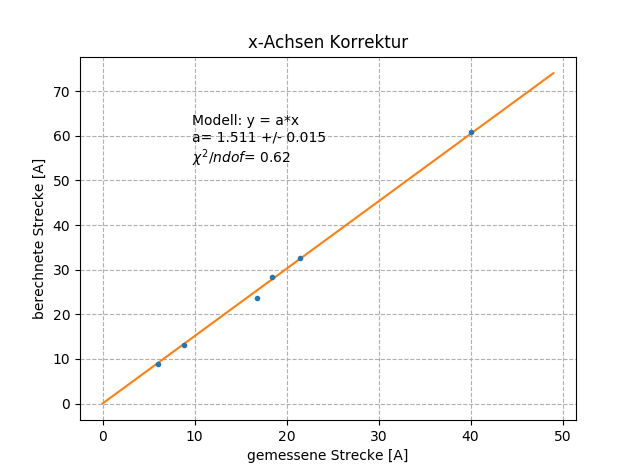
\includegraphics[scale=0.9]{Bilder/xAchse.png}
\caption{Lineare Regression anhand der Ergebnisse der x-Achsenlängen. Die Steigung a gibt den Korrekturfaktor an.}
\label{fig:strom2_abstand}
\end{figure}

\begin{figure}
\centering
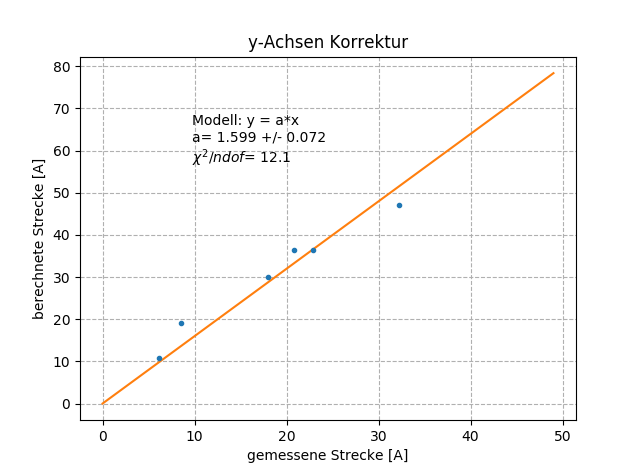
\includegraphics[scale=0.9]{Bilder/yAchse.png}
\caption{Lineare Regression anhand der Ergebnisse der y-Achsenlängen. Die Steigung a gibt den Korrekturfaktor an.}
\label{fig:strom2_abstand}
\end{figure}

\section{Fazit}

\section{Anhang}

\subsection{Achsenkorrektur Konstanthöhenmodus}
\begin{figure}[H]
\centering
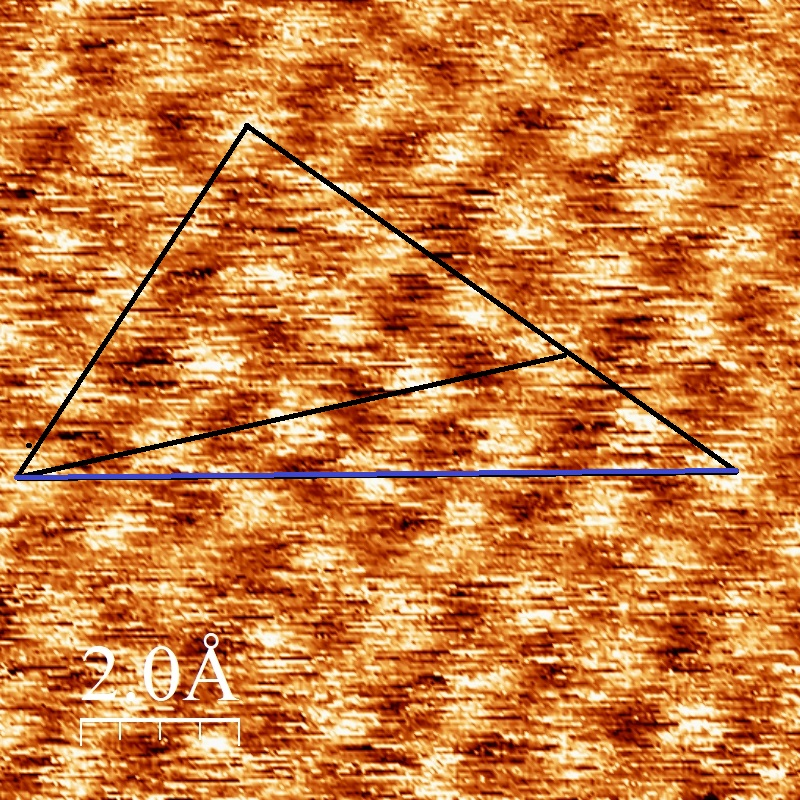
\includegraphics[scale=0.36]{Bilder/Atome/hoch1_h.jpg}
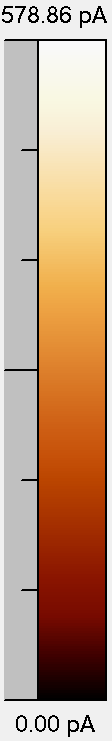
\includegraphics[scale=0.49]{Bilder/Atome/hoch1_scale.png}
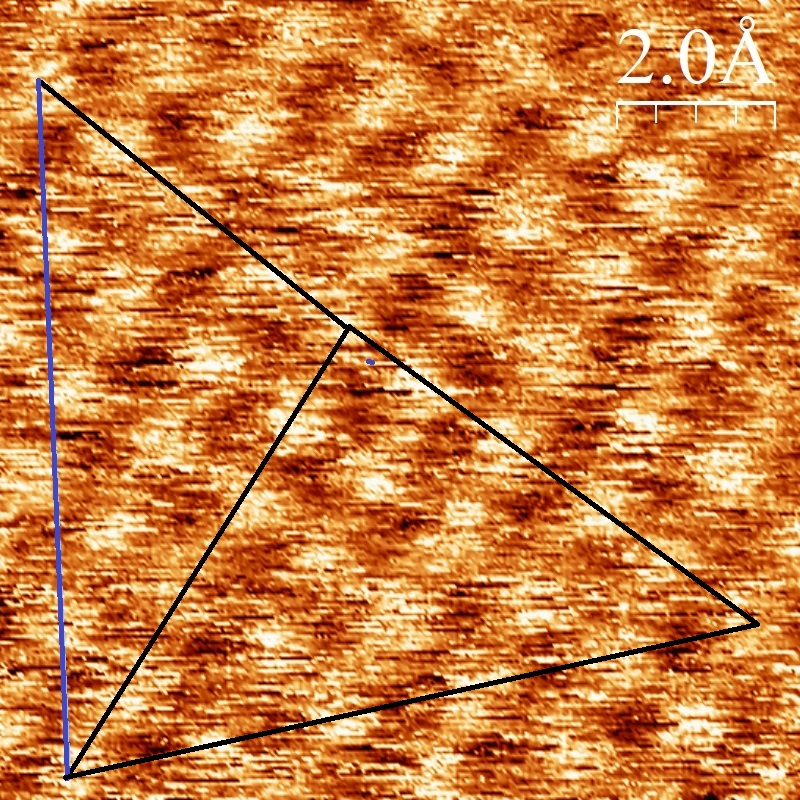
\includegraphics[scale=0.36]{Bilder/Atome/hoch1_v.jpg}
\caption{Strombild der Breite \textbf{1nm} im Konstanthöhenmodus. \textbf{Links}: Dreieck zur Bestimmung der Horizontalen Korrektur. \textbf{Rechts}: Dreieck zur Bestimmung der vertikalen Korrektur. Die blaue Linie gibt den zu bestimmenden Abstand an.}
\end{figure}

\begin{figure}[H]
\centering
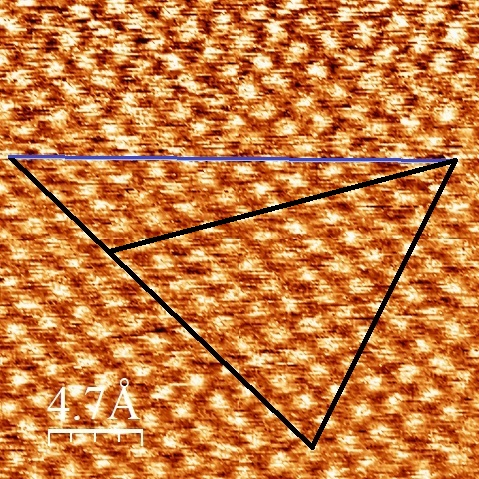
\includegraphics[scale=0.6]{Bilder/Atome/hoch2_h.jpg}
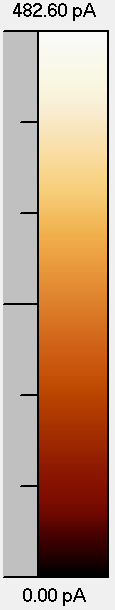
\includegraphics[scale=0.59]{Bilder/Atome/hoch2_scale.png}
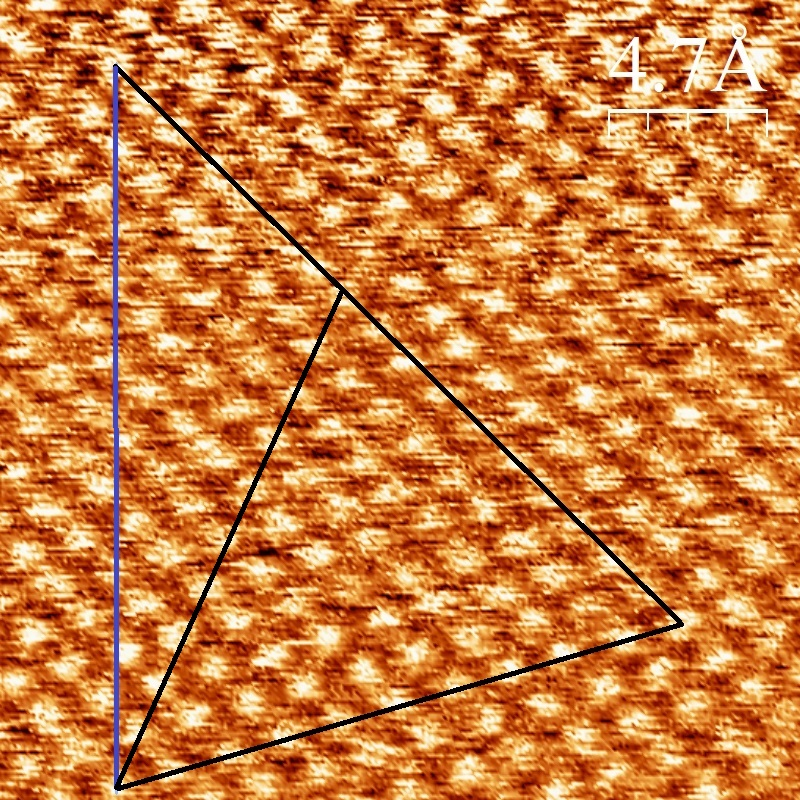
\includegraphics[scale=0.36]{Bilder/Atome/hoch2_v.jpg}
\caption{Strombild der Breite \textbf{2.325nm} im Konstanthöhenmodus. \textbf{Links}: Dreieck zur Bestimmung der Horizontalen Korrektur. \textbf{Rechts}: Dreieck zur Bestimmung der vertikalen Korrektur. Die blaue Linie gibt den zu bestimmenden Abstand an.}
\end{figure}

\begin{figure}[H]
\centering
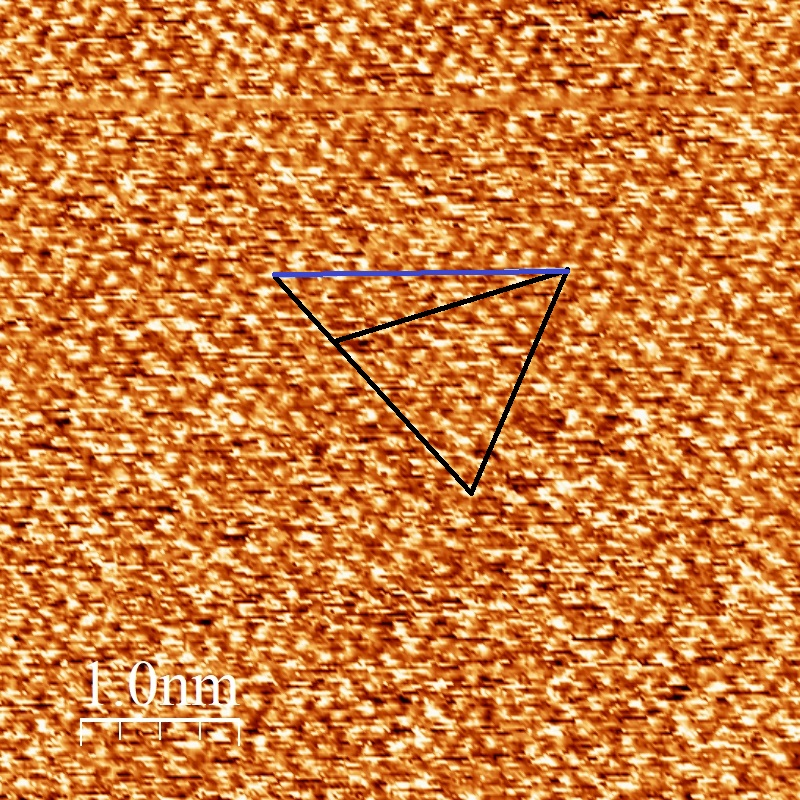
\includegraphics[scale=0.36]{Bilder/Atome/hoch5_h.jpg}
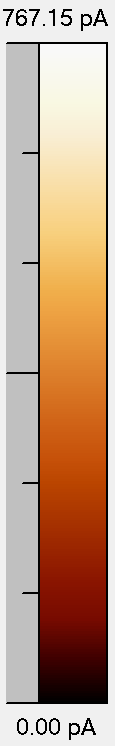
\includegraphics[scale=0.48]{Bilder/Atome/hoch5_scale.png}
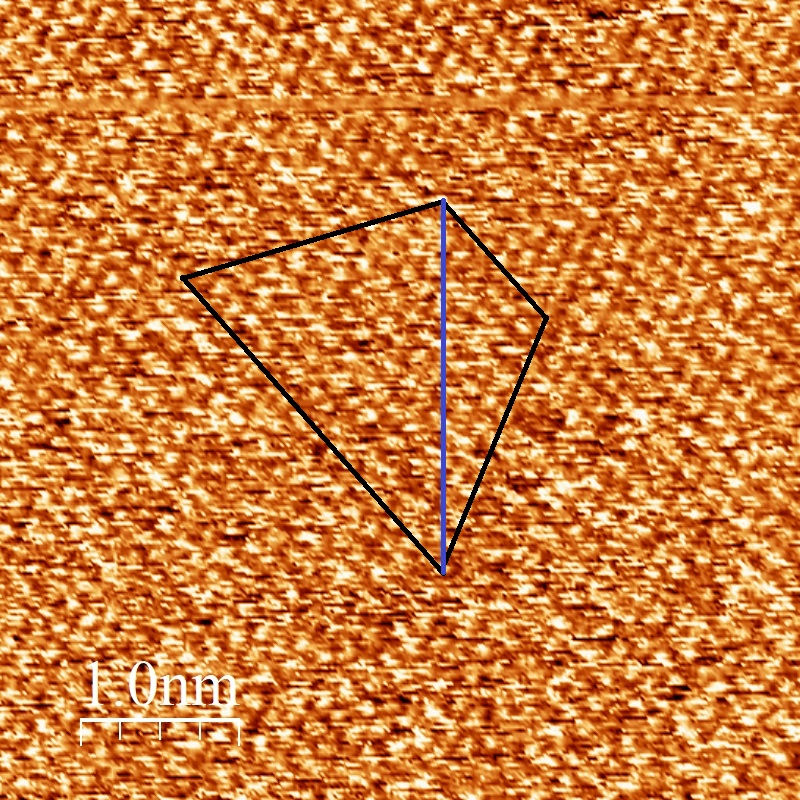
\includegraphics[scale=0.36]{Bilder/Atome/hoch5_v.jpg}
\caption{Strombild der Breite \textbf{5nm} im Konstanthöhenmodus. \textbf{Links}: Dreieck zur Bestimmung der Horizontalen Korrektur. \textbf{Rechts}: Dreieck zur Bestimmung der vertikalen Korrektur. Die blaue Linie gibt den zu bestimmenden Abstand an.}
\end{figure}

\subsection{Achsenkorrektur Konstantstrommodus}
\begin{figure}[H]
\centering
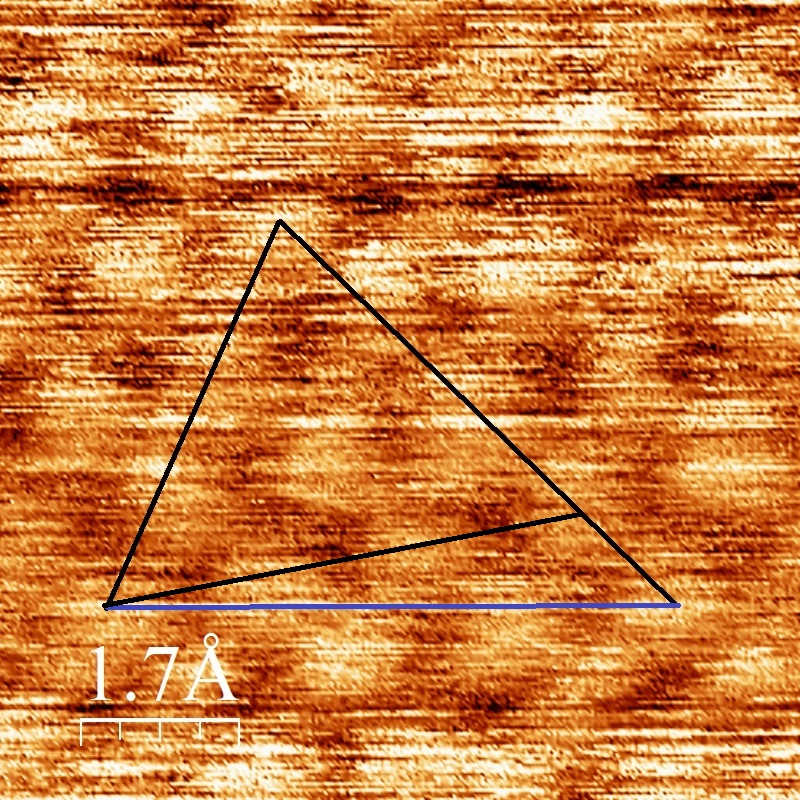
\includegraphics[scale=0.36]{Bilder/Atome/strom1_h.jpg}
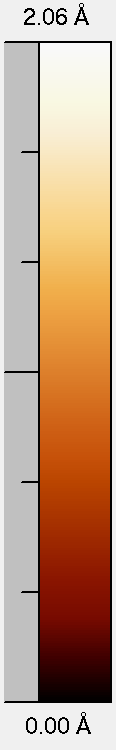
\includegraphics[scale=0.48]{Bilder/Atome/strom1_scale.png}
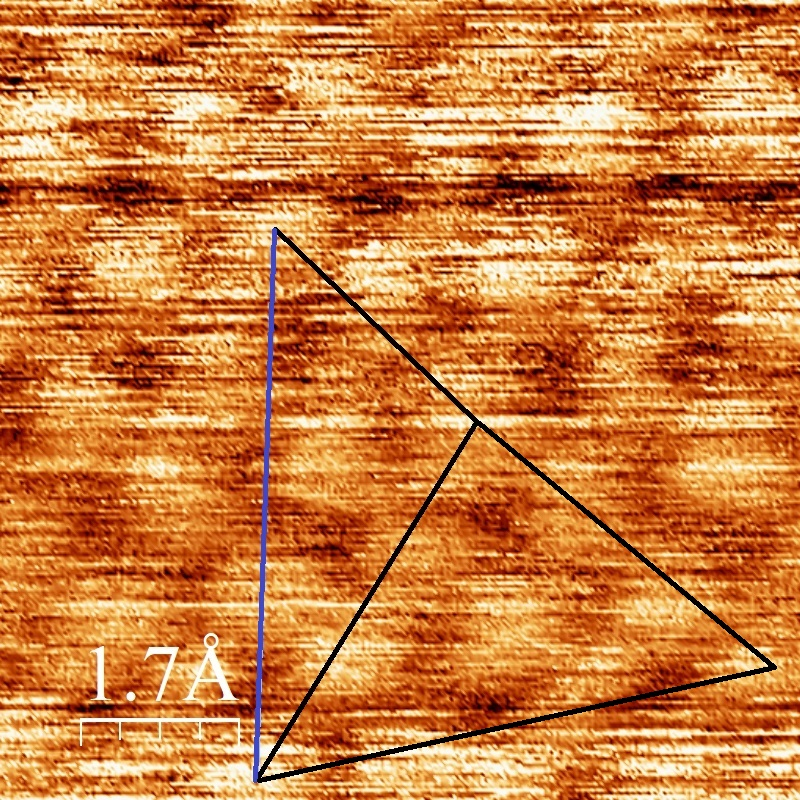
\includegraphics[scale=0.36]{Bilder/Atome/strom1_v.jpg}
\caption{Höhenprofil der Breite \textbf{0.8719nm} im Konstantstrommodus. \textbf{Links}: Dreieck zur Bestimmung der Horizontalen Korrektur. \textbf{Rechts}: Dreieck zur Bestimmung der vertikalen Korrektur. Die blaue Linie gibt den zu bestimmenden Abstand an.}
\end{figure}

\begin{figure}[H]
\centering
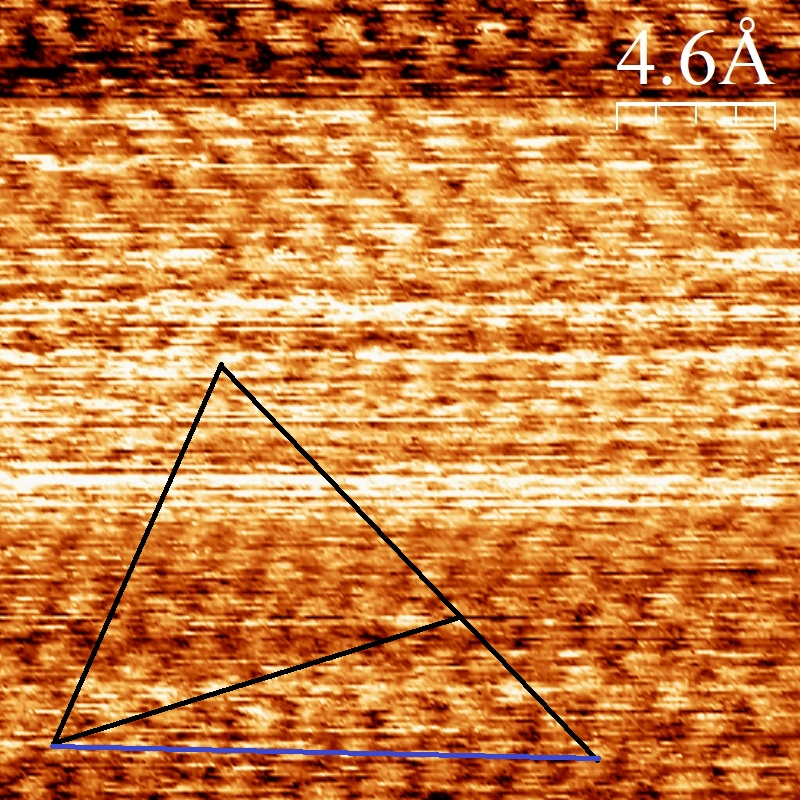
\includegraphics[scale=0.36]{Bilder/Atome/strom2_h.jpg}
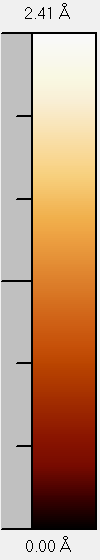
\includegraphics[scale=0.64]{Bilder/Atome/strom2_scale.png}
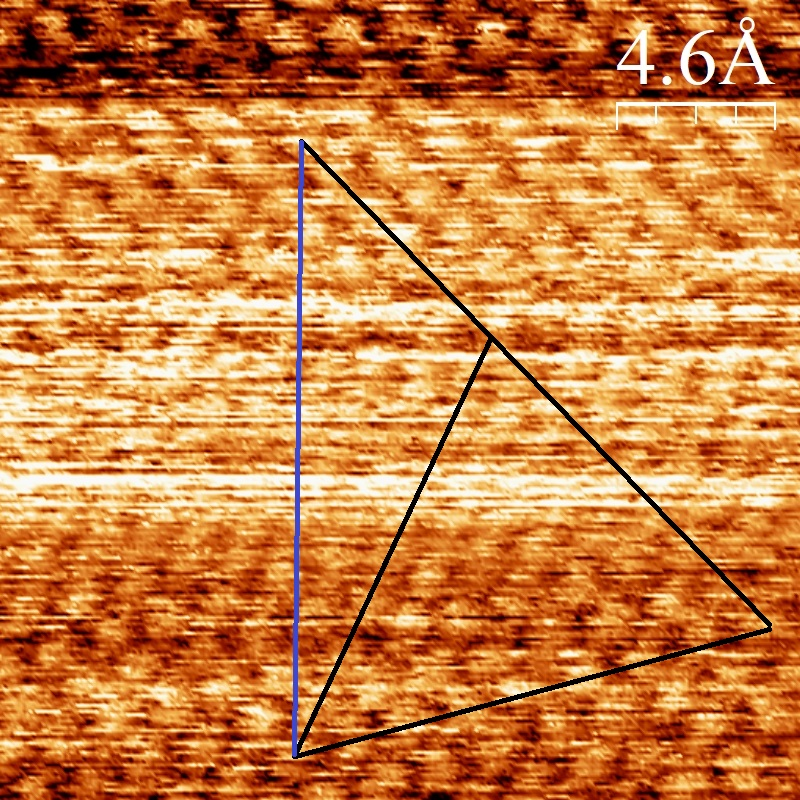
\includegraphics[scale=0.36]{Bilder/Atome/strom2_v.jpg}
\caption{Höhenprofil der Breite \textbf{2.325nm} im Konstantstrommodus. \textbf{Links}: Dreieck zur Bestimmung der Horizontalen Korrektur. \textbf{Rechts}: Dreieck zur Bestimmung der vertikalen Korrektur. Die blaue Linie gibt den zu bestimmenden Abstand an.}
\end{figure}

\begin{figure}[H]
\centering
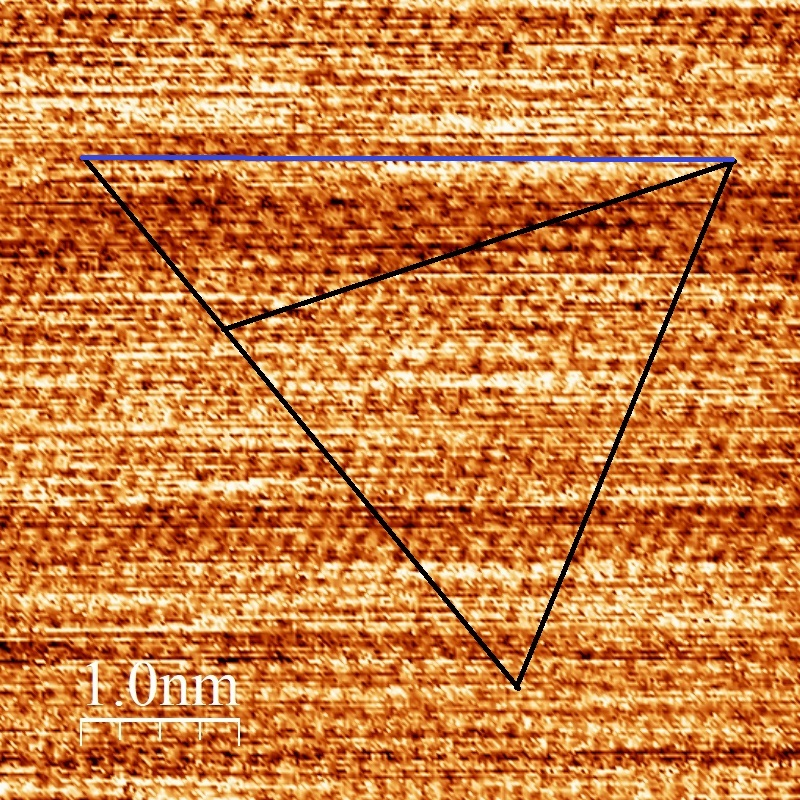
\includegraphics[scale=0.36]{Bilder/Atome/strom5_h.jpg}
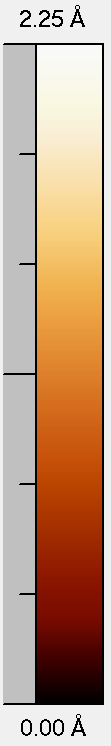
\includegraphics[scale=0.48]{Bilder/Atome/strom5_scale.png}
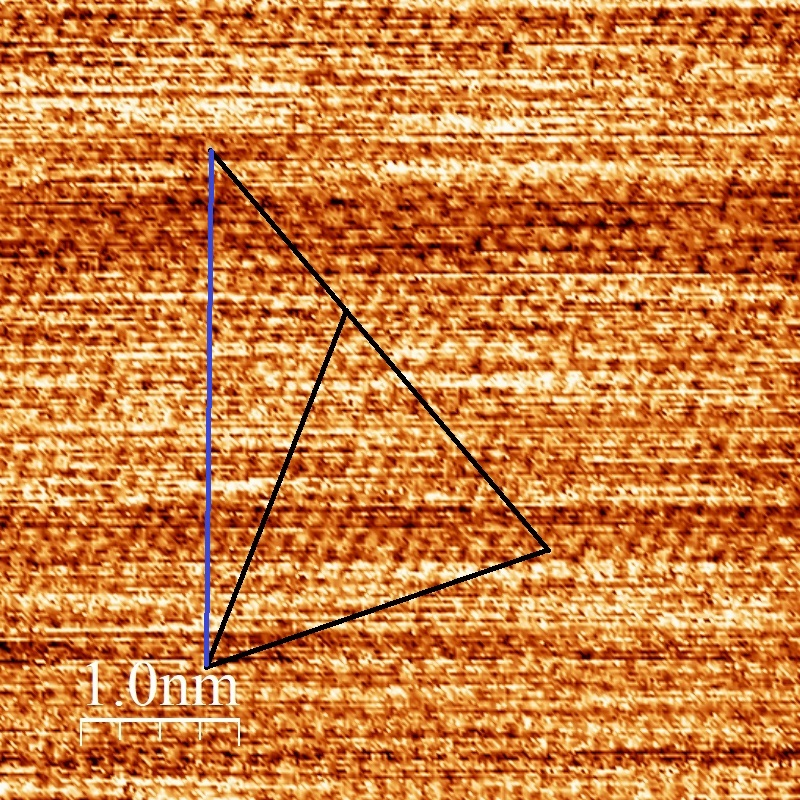
\includegraphics[scale=0.36]{Bilder/Atome/strom5_v.jpg}
\caption{Höhenprofil der Breite \textbf{5nm} im Konstantstrommodus. \textbf{Links}: Dreieck zur Bestimmung der Horizontalen Korrektur. \textbf{Rechts}: Dreieck zur Bestimmung der vertikalen Korrektur. Die blaue Linie gibt den zu bestimmenden Abstand an.}
\end{figure}

\end{document}